%Software (Arsitektur Komputer)
%Kelas : D4 TI 1B
%Khadijah Hasanah Putri Harahap 1174022
%Liyana Majdah Rahma 1174039
%Luthfi Muhammad Nabil 1174035
%Nisrina Aulia Firdaus 1174098
%Salwaa Tania 1174047
%Septia Rahayu 1174044
%Diana Satima Gistivani 1154018




\section{Definisi Software}
Software secara singkat ialah sebuah aplikasi yang terdapat pada computer maupun perangkat lunak berbasis elektronik lainnya. Fungsi dari Software sendiri cukup beragam dan mampu diterima oleh masyarakat pada umumnya. Dan berikut adalah Definisi, fungsi, bahkan Sejarah dari perkembangan Software itu sendiri.

\begin{figure}[ht]
\centerline{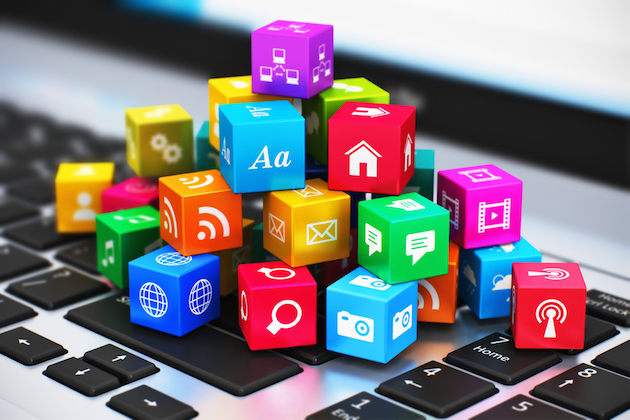
\includegraphics[width=0.5\textwidth]{figures/Abstraksi.jpg}}
\caption{Sistem Operasi}
\label{Abstraksi}
\end{figure}
\begin{flushleft}
Software adalah instruksi langsung untuk computer ataupun perangkat elektronik lain yang dapat ditemukan di berbagai tempat dan pemakaian yang beragam seperti Software sebagai pendeteksi detak jantung di rumah sakit ataupun Software hiburan seperti video games. Pada gambar \ref{Abstraksi} terlihat sebuah tampilan software Sistem Operasi. Produk Software sendiri memiliki berbagai macam jumlah kode baik dari yang hanya ratusan kode maupun jutaan kode yang diharapkan dapat melakukan pekerjaan secara efisien untuk para pengguna dari aplikasi tersebut. Software sendiri merupakan inti dari computer karena untuk mengoperasikan sebuah Komputer haruslah dalam computer tersebut memiliki perangkat keras. Software sendiri bersifat bisa terbaca namun tidak berwujud umumnya perangkat keras yang memang pada dasarnya bisa disentuh. 
\end{flushleft}
\begin{flushleft}
Software dibuat oleh seorang Perekayasa Perangkat Lunak  atau yang sering disebut sebagai Programmer. Programmer sendiri bertugas membuat sebuah Software sesuai dengan kebutuhan dari seorang klien maupun Programmer itu sendiri dan menerapkan beberapa Teknologi yang ada untuk dipakai oleh Programmer itu sendiri dan juga melakukan pemeliharaan Software yang telah dibuatnya jika Programmer tersebut diposisikan sebagai Pengembang Software. Teknik Rekayasa Software sendiri dapat meningkatkan efisiensi dan memberikan kemudahan bagi Pengembang Software dalam mengembangkan sebuah Software yang telah dibuat. 
\end{flushleft}
\begin{flushleft}
Pembuatan Software sendiri dibuat menggunakan bahasa pemrograman yang dibuat oleh programmer yang kemudian disusun (compile) sehingga membentuk kode-kode yang bisa dibaca oleh perangkat keras. Software dibuat untuk memenuhi kebutuhan – kebutuhan tertentu sesuai dengan perkembangan zaman. Software berfungsi untuk memproses data, Instruksi atau perintah yang nantinya menghasilkan sebuah hasil (Output) sesuai kebutuhan. Selain itu Software juga berfungsi sebagai penghubung antara pengguna dengan perangkat keras.
\end{flushleft}

\section{Sejarah Perkembangan Software}
\begin{flushleft}
Software telah berkembang melalui empat era yang terjadi sejak tahun 1950 sampai sekarang. Setiap era memiliki karakteristik khusus dan setiap tahunnya Software mengalami peningkatan, baik dari kompleksitas, ukuran, teknologi, dan efisiensinya dalam melakukan pekerjaan. 
\end{flushleft}
\begin{flushleft}
Krisis Software pernah terjadi pada tahun 1960 karena praktik Rekayasa Software masih kurang dapat diterima. Tahap awal Software sendiri memunculkan banyak minat pada computer, walaupun banyak kode yang ditulis, tetapi tidak ada standar yang ditetapkan. Lalu pada awal tahun 1970-an, banyak program computer mulai mengalami kegagalan dan banyak orang kehilangan kepercayaan pada sebuah Software sehingga krisis Software diumumkan. Alasan yang mengarah pada krisis adalah sebagai berikut :
\begin{itemize}
	\item Perkembangan perangkat keras yang lebih cepat
	\item Kemampuan untuk membangun yang dituntut untuk memenuhi kebutuhan secara cepat
	\item Meningkatnya ketergantungan pada Software
	\item Desain yang kurang dan minimnya teknologi maupun Sumber Daya Manusia
\end{itemize}
\end{flushleft}
\begin{flushleft}
Walaupun krisis Software teridentifikasi pada awal-awal tahun, tetapi pada tahun-tahun sebelumnya sudah pernah terjadi kegagalan Software di seluruh dunia. Software pada dasarnya di anggap gagal jika proyek pembuatan tersebut dihentikan karena faktor kekurangan biaya atau melewati jadwal yang telah ditentukan atau jika proyek melebihi 50 persen dari perencanaan. Beberapa contoh kegagalan Software mencakup kegagalan system control lalu lintas, kegagalan Software medis, kegagalan Software telekomunikasi, dan sebagainya. Alasan utama kegagalan yang lainnya adalah dikarenakan pengadopsian Praktik Rekayasa Software yang buruk. Beberapa praktik Software yang buruk meliputi : 
\begin{itemize}
	\item Tidak adanya histori pengukuran Software
	\item Penolakan dari keakuratan perkiraan daya
	\item Gagalnya penggunaan alat untuk perencanaan dan memperkirakan secara otomatis
	\item Praktik yang berlebihan
	\item Jadwal yang tidak logis
	\item Kegagalan menggunakan desain review dan inspeksi kode
\end{itemize}
\end{flushleft}
\begin{flushleft}
Untuk menghindari kegagalan dan meningkatkan kepercayaan dari masyarakat, dibutuhkan pemahaman yang baik dari proses tersebut, penyusunan jadwal yang ditargetkan untuk pembuatan sebuah Software yang terbaik dan mengukur biaya yang sebanding maupun kualitas yang dibutuhkan. Suatu proses Software merupakan serangkaian kegiatan, metode, dan praktik – praktik yang melibatkan transformasi yang dilakukan orang untuk mengembangkan dan memelihara sebuah Software. 
\end{flushleft}
\begin{flushleft}
Saat ini kebanyakan masalah terjadi dikarenakan adanya proses Software yang kacau dan terkadang keberhasilan Software tergantung pada usaha perorangan. Oleh karena itu, dibutuhkan pengalihan focus dari sebuah produk kepada proses karena terfokus kedalam produk cenderung mengabaikan masalah skalabilitas dan hanya akan melakukan perbaikan pada system yang ada. Selain itu, alasan tersebut bisa berkaitan dengan prinsip – prinsip Rekayasa Software apabila kebutuhan teridentifikasi dengan benar. Apabila identifikasinya benar, maka akan memudahkan dalam mengidentifikasi teknik atau praktik terbaik yang dapat diterapkan kepada Software karena satu proses bisa saja cocok untuk satu organisasi dan bisa tidak cocok untuk sebagian lainnya. Perkembangan dari sebuah Software berproses melalui beberapa era, diantaranya :
\begin{enumerate}
	\item Era Pioner/Pemula (Tahun 1950-1960) \\	
Dalam era ini, bentuk dari Software masih berbentuk sambungan kabel ke bagian – bagian pada computer. Pengaksesan computer sendiri masih dilakukan dengan <i>punched card</i>, yaitu kartu yang dilubangi. Penggunaan computer pada saat itu masih dilakukan secara kontak langsung. Software pada era ini masih menyatu dengan perangkat kerasnya dan hanya menghasilkan sebuah hasil berupa cetakan. Pengaplikasian pada masa ini pun masih terbilang hanya untuk keperluan yang tidak begitu banyak dikarenakan teknologi yang masih terbilang sangat kuno, seperti untuk membuat alat perhitungan matematika yang digunakan oleh ilmuwan untuk menyelesaikan operasi matematika secara cepat. 
	\item Era Stabil (Tahun 1960-1970) \\
Dalam era ini, pengguna computer sudah sangat meningkat, tidak hanya oleh kalangan peneliti tetapi juga oleh kalangan industri. Perusahaan Software pun mulai bermunculan dan sebuah Software dapat menjalankan beberapa ini. Di era ini, Software mulai bisa dibilang terpisah dari perangkat kerasnya dan bisa dikenal sebagai sebuah produk. Kode perintah Software yang dijalankan oleh computer pun tidak lagi satu-satu, tetapi sudah menampilkan banyak proses yang dilakukan secara serempak. Sebuah Software juga bisa digunakan oleh banyak pengguna secara cepat. Pada era ini juga basis data yang berfungsi menyimpan sebuah data mulai diperkenalkan.
	\item Era Mikro (Tahun 1970-1980) \\
Pada era ini, Software mulai berkembang sebagai perangkat yang dapat memenuhi kebutuhan perseorangan. Software juga dapat dibedakan menjadi Software system yang bertugas menangani sisi internal seperti Sistem Operasi dan Software aplikasi yang dapat digunakan langsung oleh penggunanya untuk keperluan tertentu. 
	\item Era Modern (Tahun 1980-Sekarang) \\
Pada era yang kita alami sekarang, Software sudah dapat dijangkau di berbagai perangkat elektronik, bahkan sebuah computer genggam atau telepon genggam terdapat sebuah aplikasi yang dapat disambungkan atau disinkronkan dengan computer. Bahkan telepon, TV, mesin cuci, dan Oven sekalipun terdapat Software yang berfungsi untuk mengatur operasi dari perangkat keras. Bahkan semua peralatan tersebut bisa dipantau dan diatur hanya menggunakan sebuah telepon genggam. Pembuatan Software bukan lagi pekerjaan yang hanya dilakukan oleh segelintir orang, tetapi telah menjadi pekerjaan banyak orang dengan teknik yang dibilang cukup memadai. Teknologi yang berkembang juga membantu orang awam untuk mempelajari bagaimana cara untuk membuat Software sendiri. Software sendiri sekarang memiliki fitur suara dan tampilan gambar.
\end{enumerate}
\end{flushleft}
\section{Dampak dari munculnya Software}
\begin{flushleft}
Software pada masa dulu dan sekarang sudah sangat mempengaruhi masyarakat dan budaya yang selalu dilakukan dalam berinteraksi ataupun melakukan sebuah pekerjaan. Seiring teknologi mulai berkembang, dampak dari munculnya Software mulai sangat drastis dibandingkan dengan tidak adanya Software. Faktor dari Software yang mempengaruhi masyarakat salah satunya yaitu : 
\begin{enumerate}
	\item Faktor Ekonomi\\
	Software pada masa emasnya memimpin produktivitas dan total nilai produksi barang. Seperti di Amerika Serikat, Software memimpin sekitar ¼ dari semua peningkatan total nilai produksi barang pada tahun 1990-an (atau sekitar 90 Miliar Dollar per tahun) dan 15 persen dari semua pertumbuhan produktivitas pada akhir tahun 1990-an (atau sekitar 33  Miliar Dollar/tahun).
	\item Faktor Sosial\\
Munculnya Software mulai mengubah budaya masyarakat yang sebagian besar mulai menggunakan computer. Dengan adanya E-mail, World Wide Web, dan pesan singkat memungkinkan orang untuk berinteraksi dengan cepat dari semua tempat terjauh sekalipun dan mengurangi biaya dari sebuah pesan singkat. 
Kesuksesan dari Software juga telah diterapkan yang mencakup Linux, Space Shuttle Software, dan Automatic Teller Machine (ATM)	
\end{enumerate}
\end{flushleft}
\section{Jenis - Jenis Software}
\begin{flushleft}
Software adalah sebuah program computer yang berfungsi sebagai penghubung antara pengguna dan perangkat keras. Software juga dapat disebut sebagai penerjemah instruksi yang dijalankan pengguna computer untuk dikirim ke perangkat keras. Software dibagi menjadi tiga bagian, yaitu program Aplikasi, Sistem Operasi, dan Bahasa Pemrograman. 
\end{flushleft}
\subsection{Software Antivirus}
\begin{flushleft}
Software ini berfungsi untuk mendeteksi dan menghapus virus computer system computer. Software ini juga dapat menentukan apakah sebuah system computer telah terinfeksi atau terdapat adanya sebuah virus atau tidak. Antivirus biasanya melakukan pemindaian secara otomatis pada system computer ke semua berkas yang bisa diakses. Pergerakan mencurigakan dari sebuah aplikasi juga dapat terdeteksi oleh Antivirus dan bisa dicurigai oleh Antivirus sebagai sebuah program yang mencurigakan. Antivirus adalah Software yang termasuk kedalam bagian dari program aplikasi.
\end{flushleft}
\subsection{Software Bisnis}
\begin{flushleft}
Software ini berfungsi sebagai program untuk melakukan sebuah pekerjaan kantoran seperti menyiapkan presentasi, membuat sebuah dokumen statistika, dan sebagainya. Aplikasi ini sangat sering digunakan oleh pekerja kantoran bahkan sampai akademisi atau pelajar masa kini. Contoh dari aplikasi yang sering digunakan adalah Microsoft Office dan Open Office.
\end{flushleft}
\subsection{Software Desain Grafis}
\begin{flushleft}
Desain Grafis juga dipermudah dengan adanya Software khusus untuk Desain Grafis di computer. Seperti Aplikasi Adobe Photoshop yang mampu mengubah gambar yang ada menjadi sesuatu sesuai keinginan sang editor. Bahkan Foto yang telah di scan dapat di edit memakai Aplikasi ini dan dapat dicetak setelahnya atau dijadikan simpanan di computer. 
\end{flushleft}
\subsection{Software Grafis 3D}
\begin{flushleft}
Dengan adanya Software ini, sebuah gambar 3 Dimensi dapat dibuat bahkan dapat digerakkan seperti film anak – anak yang menggunakan karakter 3 Dimensi atau Pembuatan kerangka bangunan 3 Dimensi. Aplikasi yang sering dipakai saat ini adalah AutoCAD atau 3DS Max yang dikembangkan oleh Autodesk. AutoCAD banyak digunakan oleh Insinyur Sipil, Pengembang lahan, Desainer, Animator, dan lain – lain. 
\end{flushleft}
\subsection{Software Grafis}
\begin{flushleft}
Seperti halnya dengan Software Desain Grafis hanya saja Software Grafis dipakai untuk membuat sebuah grafis visual seperti diagram aliran (flowchart), brainstorm, dan Skema Jaringan. Contoh dari aplikasi Software Grafis seperti Microsoft Visio yang dibuat oleh Visio Corporation yang diakuisisi oleh Microsoft. Sebagian besar yang memakai aplikasi ini adalah seorang perancang sebuah proyek. 
\end{flushleft}
\subsection{Software Jaringan}
\begin{flushleft}
Dengan ketersediaan sebuah Jaringan membuat informasi yang ada di sebuah Website atau sebuah komunikasi melalui pesan singkat atau surat elektronik (E-Mail) mulai bermunculuan. Bahkan aplikasi Chatting seperti Yahoo! Messengger dan AOL mulai meledak penggunaannya karena dapat melakukan Chatting secara langsung (Realtime). Pemakai dari aplikasi ini sangat banyak digunakan oleh kalangan masyarakat.
\end{flushleft}
\subsection{Software Kompresi Data}
\begin{flushleft}
Software ini berfungsi sebagai pengompres sebuah file/data yang besar maupun mengelompokkan file – file kecil menjadi satu Archive yang berukuran lebih kecil dari total semua file kecil. Aplikasi ini banyak digunakan karena mampu membuat atau mengorganisir file – file biasa menjadi satu file berformat Archive. Contoh aplikasinya seperti WinZip, WinRAR.
\end{flushleft}
\subsection{Software Musik}
\begin{flushleft}
Untuk musik pun ada Software yang khusus untuk Memutar bahkan mengubah Musik. Tidak hanya pada computer, bahkan telepon genggam pun terdapat aplikasi Pemutar Musik. Dengan adanya aplikasi ini kita tidak perlu memutar sebuah Tape atau Cakram untuk mendengarkan atau menyimpan musik melainkan cukup menyimpan atau mendownload musik dari Jaringan Internet dan memutarnya menggunakan aplikasi musik. Pengguna aplikasi ini banyak di kalangan masyarakat pengguna computer manapun.
\end{flushleft}
\subsection{Software Pembaca Gambar}
\begin{flushleft}
Di setiap Sistem Operasi saat ini sudah banyak memiliki sebuah Software Pembaca Gambar. Gambar sendiri bisa berupa Foto atau Gambar Digital. Dengan aplikasi ini kita dapat melihat gambar di dalam computer. Aplikasi yang sering dipakai untuk melihat gambar seperti Windows Photo Viewer.
\end{flushleft}
\subsection{Software Sistem Operasi}
\begin{flushleft}
Pada era sekarang sebuah Software mulai sangat tidak berwujud atau bisa tersentuh melainkan telah diaplikasikan ke dalam computer. Sistem Operasi sendiri adalah penghubung antara sebuah Software program aplikasi dengan Perangkat Keras pada computer. Dengan adanya Sistem Operasi cukup memudahkan seorang pengembang Software untuk mengembangkan aplikasi yang telah dibuat dan mempermudah masyarakat untuk menjalankan banyak Software secara serentak sesuai dengan kemampuan sebuah computer. Sistem Operasi yang sangat dipakai sekarang adalah Sistem Operasi Windows.
\end{flushleft}
\section{Rangkuman}
\begin{flushleft}
Software telah berkembang dimulai pada tahun 1950 sampai saat ini yang pernah melalui empat  era. Setiap era memiliki peningkatan dan krisis baik dalam ukuran, kompleksitas, maupun kepercayaan masyarakat terhadap Software. Saat ini kebanyakan masalah terjadi dikarenakan proses Software yang kacau bahkan lewatnya jadwal pembuatan membuat sebuah aplikasi dianggap gagal oleh masyarakat. Oleh karena itu, suatu focus pada proses sangat dibutuhkan karena focus pada produk cenderung hanya memperbaiki system yang ada dan mengabaikan masalah skalabilitas.
\end{flushleft}
\begin{flushleft}
Perkembangan Ilmu Pengetahuan dan Teknologi berperan besar sebagai pengubah teknik pembuatan seorang Perekayasa Perangkat Lunak sampai sekarang. Pada saat ini orang tidak perlu  sangat mempermasalahkan sebuah perangkat keras untuk membuat sebuah Software melainkan hanya memperlukan Ilmu yang cukup untuk dapat menggunakan bahasa pemrograman yang akan dikonversi ke bahasa computer. 
\end{flushleft}
\begin{flushleft}
Dengan adanya Software memudahkan masyarakat dalam melakukan pekerjaan tertentu dan bahkan bisa membersihkan sebuah system computer yang terinfeksi oleh sebuah virus. Fungsi dari Software sendiri sudah dipakai oleh Masyarakat biasa sampai Ilmuwan ataupun seorang Dinas social Masyarakat. Jenis – jenis Software juga sangatlah beragam dimulai dari Software Antivirus sebagai Pelindung Sistem Komputer sampai Software Sistem Operasi sebagai penghubung antara Software dan perangkat keras.
\end{flushleft}
Sumber dari artikel dipetik dari buku \cite{simarmata2010rekayasa}
